%% 20250606: DOES NOT COMPILE
%\documentclass[nooutcomes]{ximera}
%%% \input{../otherpreamble.tex}
\author{Elizabeth Miller}
\license{Creative Commons Attribution 4.0 International License}
\acknowledgement{https://spot.pcc.edu/math/orcca/ed2/html/section-exploring-two-variable-data-and-rate-of-change.html}

\title{Linear Equations: Equations of Lines}

\begin{document}
\begin{abstract}
  We explore the different ways we might write the equation of a line including the slope-intercept form, the point-slope form, and standard form.
\end{abstract}
\licenseORCCA
\maketitle
We will explore how to write an equation for a line.  The best way to write the equation of a line depends both on what information we have about the line and what we want to do with our equation.  

%\typeout{************************************************}
%\typeout{Slope-Intercept Form of a Line}
%\typeout{************************************************}

\section{Slope-Intercept Form of a Line}

Recall the previous example where Yara had \$50 in her savings account when the year began, and decided to deposit \$20 each week without withdrawing any money. In that example, we model using $x$ to represent how many weeks have passed. After $x$  weeks, Yara has added $20x$ dollars. And since she started with \$50,  she has

$$y=20x+50$$ 

in her account after $x$ weeks. In this example, there is a constant rate of change of 20 dollars per week, so we call that the slope. We also saw that plotting Yara's balance over time gives us a straight-line graph.

\begin{objectives}\begin{itemize}
  \item Me
  \item me too
  \end{itemize}
\end{objectives}



\begin{objectives}Blah\begin{itemize}
  \item Me
  \item me too
  \end{itemize}
\end{objectives}



\begin{image}
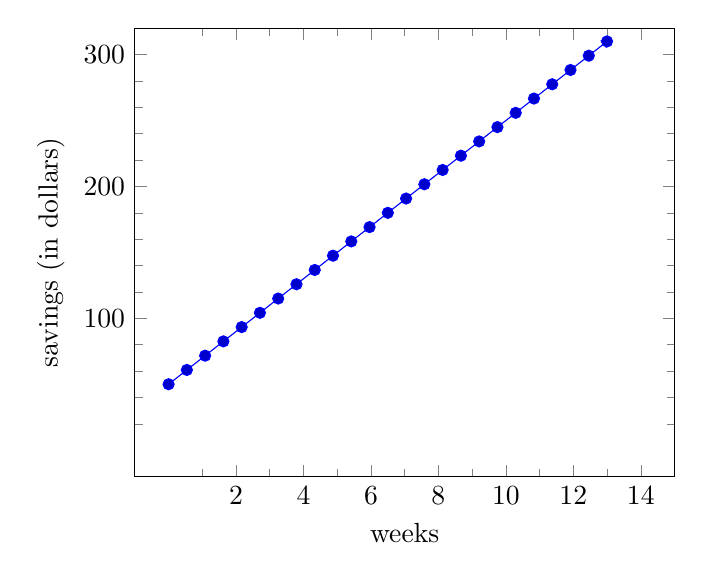
\begin{tikzpicture}
    \begin{axis}[xlabel={weeks},
                ylabel={savings (in dollars)},
                xmin=-1,xmax=15,
                ymin=-20,ymax=320,
                xtick={2,4,...,14},
                minor xtick={1,2,...,15},
                ytick={100,200,300},
                minor ytick={20,40,...,320},
                ]
        \addplot+[domain = 0:13,->]{50+20*x};
    \end{axis}
  \end{tikzpicture}
\end{image}

The graph of Yara's savings has some things in common with almost every straight-line graph. There is a slope, and there is a place where the line crosses the 
y
-axis. We use the symbol, $m$, for the slope of a line. 

\begin{image}
\begin{tikzpicture}
    \begin{axis}[ticks=none,grid=none]
        \addplot+[] {0.5*x+2} node[pos=0.8,sloped,above] {slope};
        \addplot[soliddot] coordinates {(0,2)} node[above left] {$y$-intercept};
    \end{axis}
\end{tikzpicture}
\end{image}


\begin{definition}
The $y$-intercept is a point on the $y$-axis where the line crosses. Since it's on the $y$-axis, the $x$-coordinate of this point is 0.   It is standard to call the point $(0,b)$ the $y$-intercept, and call the number $b$ the $y$-coordinate of the $y$-intercept.
\end{definition}

One way to write the equation for Yara's savings was $$y=20x+50$$ where both $m=20$ and $b=50$ are immediately visible in the equation. Now we are ready to generalize this.


\begin{definition}
When $x$ and $y$ have a linear relationship where $m$  is the slope and $(0,b)$ is the $y$-intercept, one equation for this relationship is $$y=mx+b$$ and this equation is called the \textbf{slope-intercept form} of the line. It is called this because the slope and $y$-intercept are immediately discernible from the numbers in the equation.
\end{definition}


\begin{problem}
What is the slope and $y$-intercept for the line with the following linear equation?
$$y=17x-14$$

Slope = $\answer[given]{17}$
$y$-intercept=$(0,\answer[given]{-14})$
\begin{hint}
Note that since the formula for slope-intercept form of a line has a "+" between the $mx$ and the $b$, this means that an equation like $y=17x-14$ needs to looked at like $y=17x+(-14)$ so that it matches the formula for the slope-intercept form of a line.
\end{hint}

\end{problem}


\begin{remark}
The number $b$ is the $y$-value when $x=0$. Therefore it is common to refer to $b$ as the \textbf{initial value} or \textbf{starting value} of a linear relationship.
\end{remark}



%\typeout{************************************************}
%\typeout{Point-Slope Form of a Line}
%\typeout{************************************************}

\section{Point-Slope Form of a Line}

In the previous section, we learned that a linear equation can be written in slope-intercept form, $y=mx+b$. This section covers an alternative that is often more useful, especially in Calculus: point-slope form.

\begin{example}
Starting in 1990, the population of the United States has been growing by about 2.865  million people per year. Also, back in 1990, the population was 253 million. Since the rate of growth has been roughly constant, a linear model is appropriate. Let's try to write an equation to model this.

\begin{explanation}
We consider using $y=mx+b$, but we would need to know the $y$-intercept, and nothing in the background tells us that. We'd need to know the population of the United States in the year 0, before there even was a United States.

We could do some side work to calculate the $y$-intercept, but let's try something else. Here are some things we know:
\begin{enumerate}
\item The slope equation is $m=\frac{y_2-y_1}{x_2-x_1}$
\item The slope is $m=2.865 \frac{\text{million people}}{\text{year}}$
\item One point on the line is $(1990,253)$ because in 1990, the population was 253 million.
\end{enumerate}

If we use the generic $(x,y)$ to represent a point \textit{somewhere} on this line, then the rate of change between $(1990,253)$ and $(x,y)$  has to be 2.965.  So

$$\frac{y-253}{x-1990}=2.865$$.

While this is an equation of a line, we might prefer to write the equation without using a fraction.  Multiplying both sides by $(x-1990)$ gives us

$$y-253=2.865(x-1990)$$

This is a good place to stop. We have isolated $y$, and three meaningful numbers appear in the equation: the rate of growth, a certain year, and the population in that year. This is a specific example of point-slope form. 
\end{explanation}
\end{example}

\begin{definition}
When $x$ and  $y$ have a linear relationship where $m$ is the slope and $(x_0,y_0)$ is some specific point that the line passes through, one equation for this relationship is 
$$y-y_0=m(x-x_0)$$ 
and this equation is called the \dfn{point-slope form} of the line. It is called this because the slope and one point on the line are immediately discernible from the numbers in the equation.

\begin{image}
\begin{tikzpicture}
    \begin{axis}[xmin=-1,xmax=9,width=0.47\linewidth,
                ymin=-1,ymax=9,
                ticks=none,
                grid=none]
        \addplot+[domain = -1:9]{2/7*(x-5)+4} node[pos=0.5,above,sloped] {$y-y_0=m\left(x-x_0\right)$};
        \addplot[soliddot] coordinates {(5,4)} node[below right] {$\left(x_0,y_0\right)$};
    \end{axis}
\end{tikzpicture}
\end{image}

\end{definition}


Sometimes, it is helpful to be able to express our equation as $y=...$.  To do this when working with the Point-Slope form of a line, all you have to do is add $y_0$ to both sides of the equation.  This will give us the Alternate Point-Slope Form.  


\begin{definition}
When $x$ and  $y$ have a linear relationship where $m$ is the slope and $(x_0,y_0)$ is some specific point that the line passes through, one equation for this relationship is 
$$y=m(x-x_0)+y_0$$ 
and this equation is called the \dfn{(alternate) point-slope form} of the line. It is called this because the slope and one point on the line are immediately discernible from the numbers in the equation.
\end{definition}


Note that some people may call this second form the Point-Slope Form of a line.  Both ways of writing this form have the advantage that they can be easily written down if you just know a point on the line and the slope of the line.

%\typeout{************************************************}
%\typeout{Standard Form of a Line}
%\typeout{************************************************}

\section{Standard Form of a Line}

We've seen that a linear relationship can be expressed with an equation in Slope-Intercept form or with an equation in Point-Slope form. There is a third form that you can use to write line equations. It's known as standard form.

Imagine trying to gather donations to pay for a \$10,000 medical procedure you cannot afford. Oversimplifying the mathematics a bit, suppose that there were only two types of donors in the world: those who will donate \$20 and those who will donate \$100.

How many of each, or what combination, do you need to reach the funding goal? As in, if $x$ people donate \$20 and $y$ people donate \$100, what numbers could $x$ and $y$ be? The donors of the first type have collectively donated $20x$ dollars, and the donors of the second type have collectively donated $100y$.  

So altogether you'd need

$$20x+100y=10000$$

This is an example of a line equation in standard form.


\begin{definition}
 It is always possible to write an equation for a line in the form
$$Ax+By=C$$
where $A$,$B$, and $C$ are three numbers (each of which might be 0, although at least one of $A$ and $B$ must be nonzero). This form of a line equation is called \dfn{standard form}. 
\end{definition}


In the context of an application, the meaning of $A$, $B$,  and $C$ depends on that context. This equation is called standard form perhaps because any line can be written this way, even vertical lines (which cannot be written using slope-intercept or point-slope form equations).


\section{Special Lines}
While we can write the equation of a line in different forms, it is important to note that we can easily rearrange a line given in one form to another form using algebra.

There are two special types of lines which it is worth mentioning at this point.   


\begin{definition}
A \dfn{horizontal line} is a line where all the $y$-values of the points are the same.  In this case, if the $y$-value is $y_0$, then the line can be written as 
$$y=y_0$$
\begin{center}
 \begin{tikzpicture}
    \begin{axis}[xmin=-1,xmax=9,width=0.47\linewidth,
                ymin=-1,ymax=9,
                ticks=none,
                grid=none]
        \addplot+[domain = -1:9]{4} node[pos=0.5,above,sloped] {$y=y_0$};
        \addplot[soliddot] coordinates {(5,4)} node[below right] {$\left(x_0,y_0\right)$};
    \end{axis}
\end{tikzpicture}
\end{center}
\end{definition}



\begin{definition}
A \dfn{vertical line} is a line where all the $x$-values of the points are the same.  In this case, if the $x$-value is $x_0$, then the line can be written as 
$$x=x_0$$
\begin{center}
 \begin{tikzpicture}
    \begin{axis}[xmin=-1,xmax=9,width=0.47\linewidth,
                ymin=-1,ymax=9,
                ticks=none,
                grid=none]
        \addplot+[] coordinates {(3,-1) (3,9)}; {$x=x_0$};
        \addplot[soliddot] coordinates {(3,4)} node[below right] {$\left(x_0,y_0\right)$};
    \end{axis}
\end{tikzpicture}
\end{center}
\end{definition}


\end{document}
